
\chapter{Einleitung}

\begin{figure}[h]
  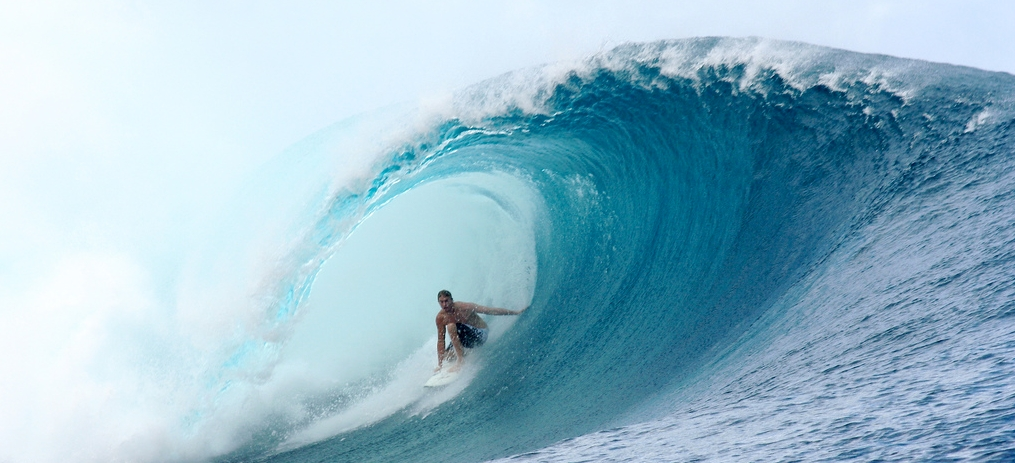
\includegraphics[width=\textwidth]{bilder/intro}
\end{figure}

\section{Surfen - Eine Wassersportart}
Mit Surfen oder Wellenreiten bezeichnet man eine Wassersportart, bei
der versucht wird, eine brechende Welle mit einem Surfbrett im Stehen
entlang zu fahren. Anders als beim Windsurfen wird hier nicht die
Kraft des Windes, sondern die Kraft der brechenden Welle benutzt, um
die zum Aufstehen und Fahren benötigte Geschwindigkeit zu
erreichen. Zum Surfen geeignete Wellen fangen idealerweise an einem
Punkt an zu brechen und fallen dann kontinuierlich in eine oder beide
Richtungen in sich zusammen. Der Surfer versucht die Welle kurz vor
dem brechenden Punkt zunächst anzupaddeln, dann so schnell wie möglich
aufzustehen, um anschließend auf der Welle so lange wie möglich in die
brechende Richtung zu fahren.

Surfbare Wellen sind allerdings nicht immer dort anzutreffen, wo es
ein Meer oder einen Strand gibt. Vielmehr sind für Surfer interessante
Wellen an den Orten zu finden, im folgenden \textit{Spots} genannt,
deren geografische Lage das Eintreffen von Wellen begünstigt, die weit
entfernt entstanden und viele Kilometer weit gereist sind. Diese Art
von Wellen wird \textit{Swell} oder auch Dünung genannt und ist eine
der Grundvoraussetzung für gute Surfbedingungen. Die Beschaffenheit
des Untergrunds, über dem Wellen anfangen zu brechen, ist ein weiterer
wichtiger Faktor, der die Qualität der zu surfenden Wellen
beeinflusst. An den bei Surfern sehr beliebten \textit{Pointbreaks}
brechen die Wellen immer an der gleichen Stelle. An diesen Spots
treffen die Wellen meist auf ein Riff oder einen aus Steinen
bzw. Felsen bestehenden Untergrund, der sie abbremst und zum Brechen
bringt. Dies sind die beständigsten, am besten einschätzbaren, aber
auch gefährlichsten Spots. Besteht der Untergrund aus Sand, sind meist
sich durch Gezeiten, Strömungen und Stürme ständig verändernde
Sandbänke für das Brechen der Wellen verantwortlich. Diese Spots sind
weniger beständig und verändern sich durch die Meeresströmung im Laufe
der Zeit sehr viel schneller als die weitaus beständigeren
\textit{Pointbreaks}.

Weitere wichtige Faktoren, die sich auf die Eigenschaften von
surfbaren Wellen auswirken, sind die Gezeiten, die Richtung aus der
die Wellen kommen sowie die Wind- und Wetterverhältnisse in den
jeweiligen Jahreszeiten. Insbesondere die Windstärke und die
Windrichtung sind hier von großem Interesse. Potentiell surfbare
Wellen können durch starken Wind aus der falschen Richtung sehr
schnell zunichte gemacht werden. Die Ausrichtung eines Spots spielt
dabei ebenfalls eine Rolle, da je nach Windrichtung einige der Spots
windgeschützter sind als andere.

Da surfbare Wellen von vielen Faktoren beeinflusst werden,
beschäftigen sich die meisten Surfer vor und während ihrer Reisen
insbesondere mit den aktuellen Wetter- und Wellenvorhersagen und
versuchen herauszufinden, welche Spots bei welchen Verhältnissen am
besten brechen. Der typische Surfer liegt deshalb nicht nur am Strand
herum und wartet dort auf gute Wellen, sondern ist oft auf abgelegenen
Straßen und Trampelpfaden entlang der Küste unterwegs, in der
Hoffnung, einen abgelegenen Spot mit den perfekten Wellen zu finden.

\section{The Stormrider Guides}
Die sogenannten \textit{Stormrider Guides} des \textit{Low Pressure}
\footnote{\url{http://www.lowpressure.co.uk}} Verlags sind seit langem
die populärsten Reiseführer in der Surfszene. Sie erfreuen sich dank
der vielen hilfreichen Informationen und Tipps rund ums Surfen einer
sehr großen Beliebtheit. Insbesondere die detaillierten Informationen
über die Eigenschaften der Wellen an den Spots sind dabei von großem
Nutzen. Die nach Kontinenten, Ländern und Regionen gegliederten Bücher
enthalten Reiseinformationen über Land und Leute, die Kultur des
Landes, das dort herrschende Klima sowie Kartenausschnitte mit
Beschreibungen zu den Surfbedingungen an den Spots. Die Bücher sind
mit qualitativ hochwertigen und teilweise spektakulären Bildern,
sowohl aus heutigen als auch aus vergangenen Zeiten illustriert.

\begin{figure}[h]
  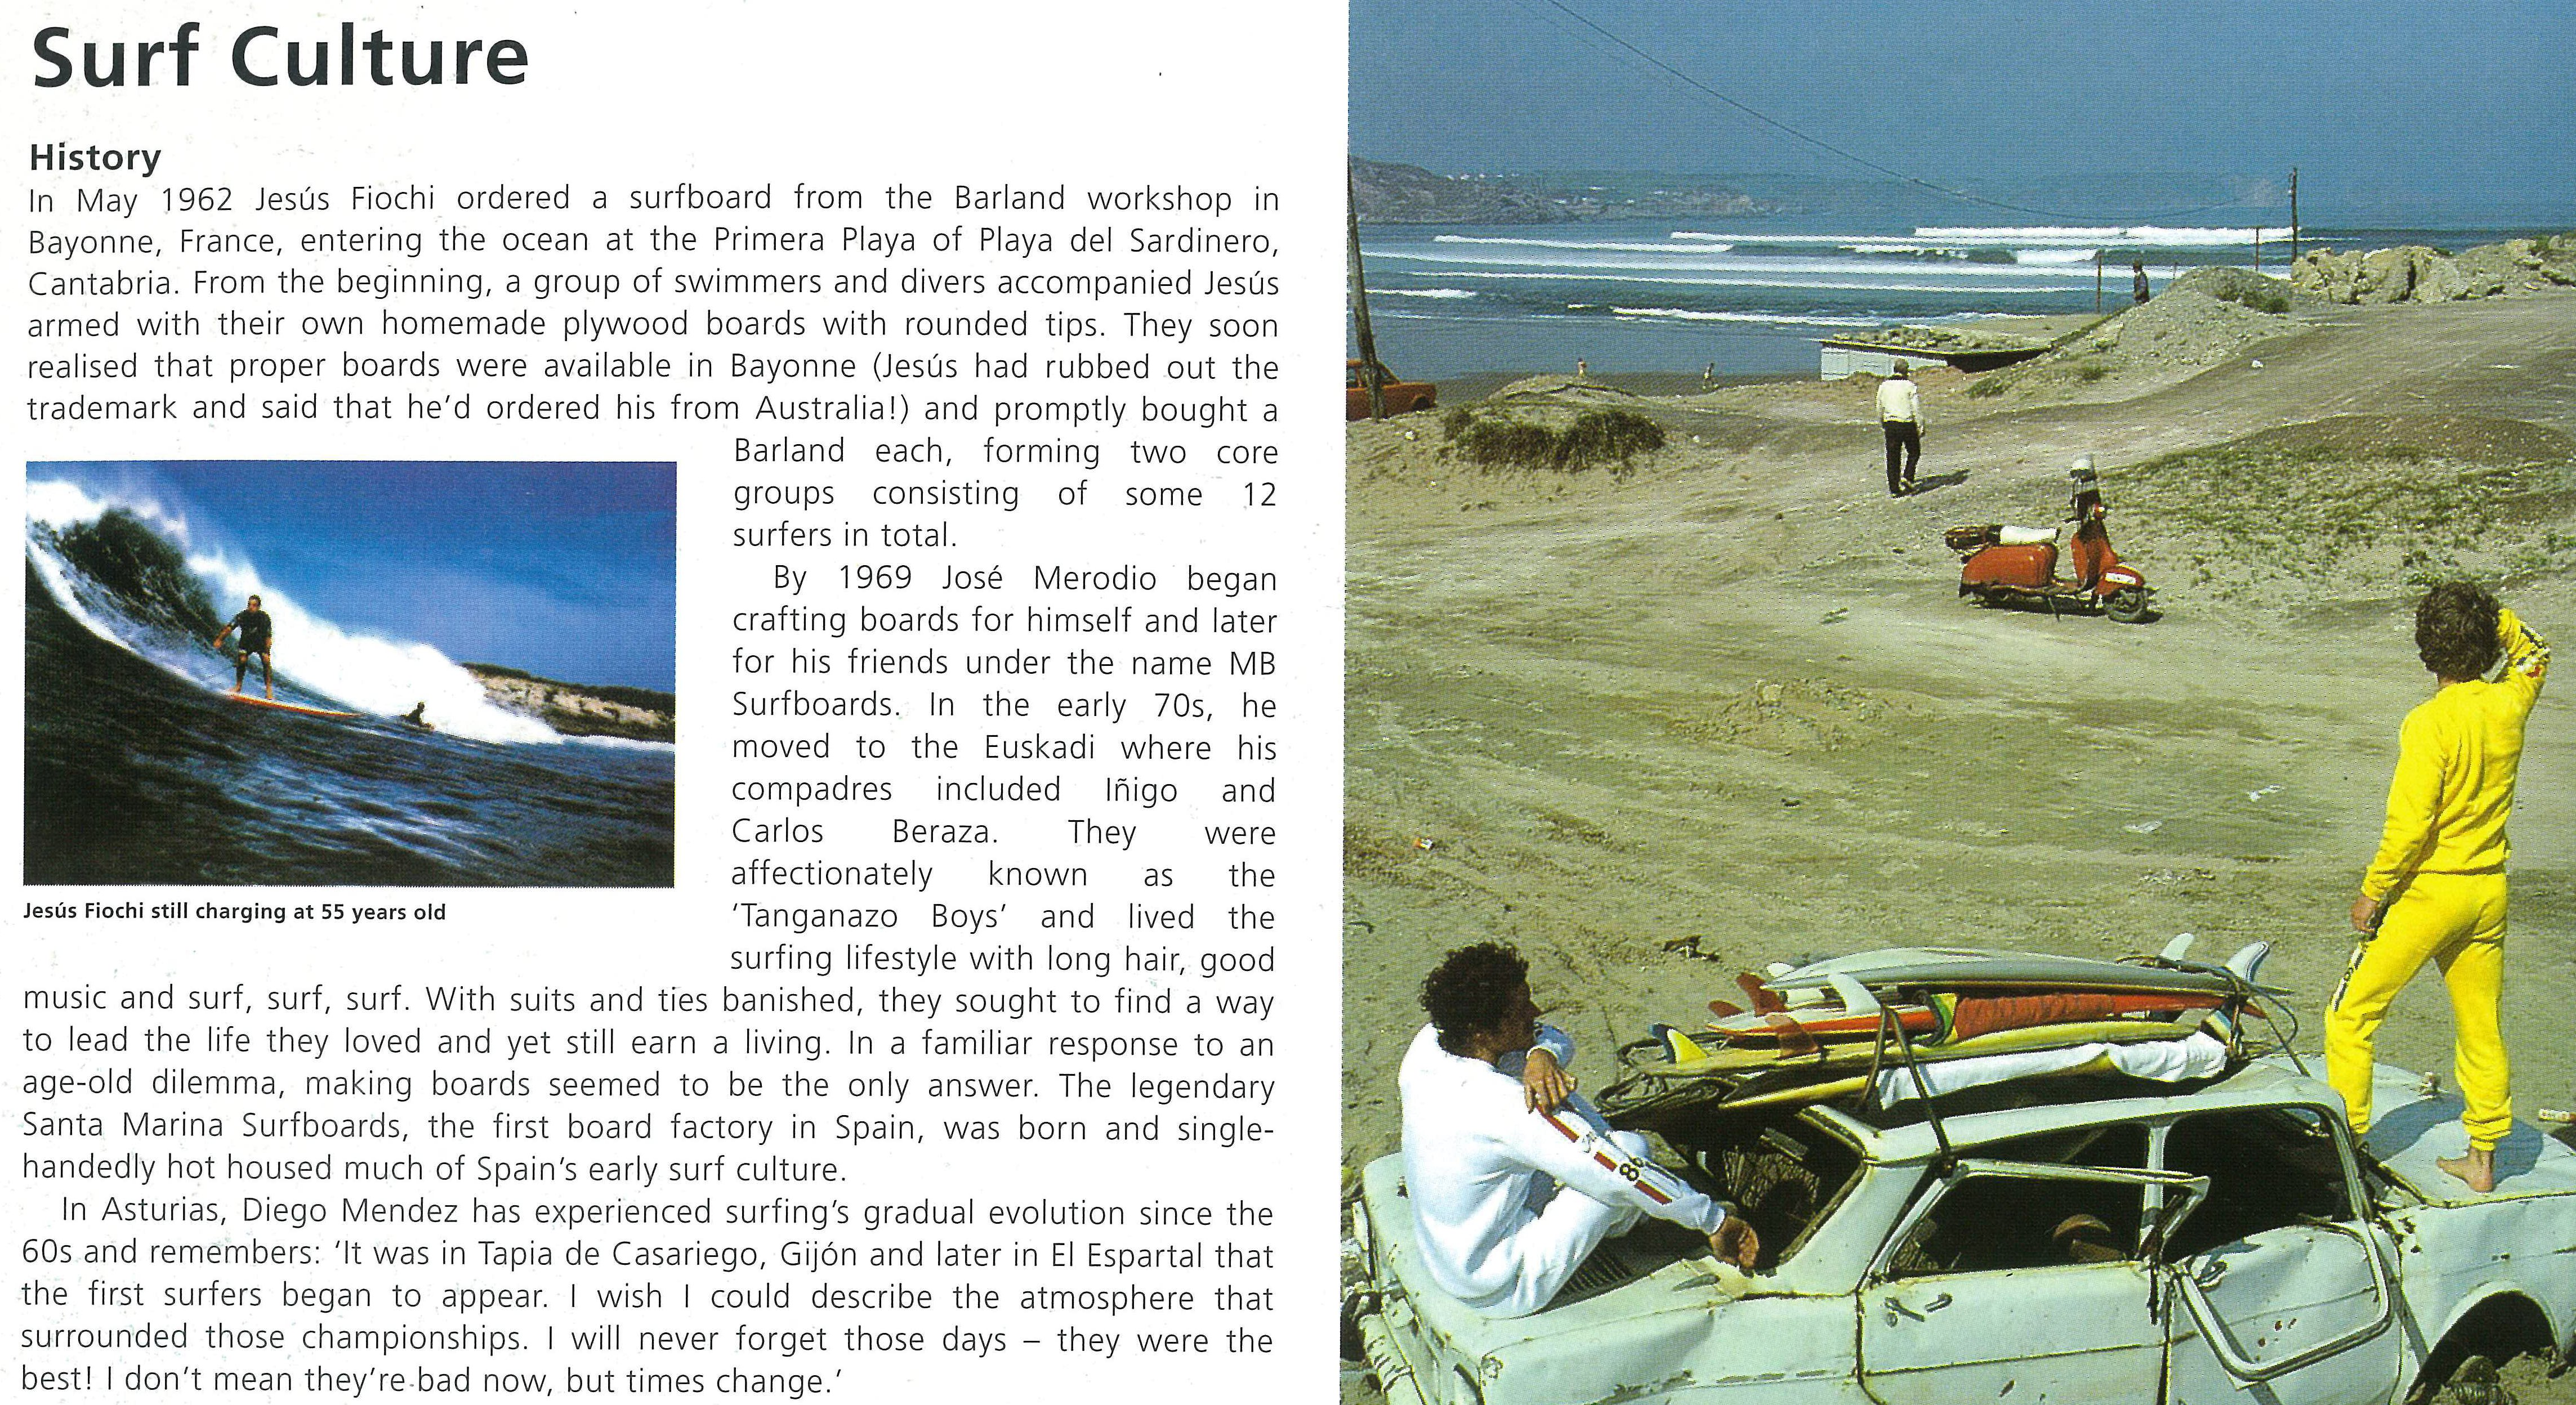
\includegraphics[width=\textwidth]{bilder/surf-culture}
  \caption{Ausschnitt zur Geschichte der Surf Kultur in Spanien}
  \label{surf-culture}
\end{figure}

In den Reiseführern ist jedem der darin beschriebenen Länder ein
eigenes Kapitel gewidmet, in denen zunächst auf die Geschichte und die
Entwicklung des Surfens in dem jeweiligen Land eingegangen wird. In
Abbildung \ref{surf-culture} ist z.B. ein Ausschnitt aus dem
\textit{Stormrider Guide Europe} zu sehen, in dem die Anfänge des
Surfens in Spanien beschrieben werden. Anschließend werden die am Meer
liegenden Regionen eines Landes vorgestellt und allgemeine Aussagen
über die dort herrschenden Surfbedingungen getroffen. Dabei werden
unter anderem die Wasser- und Lufttemperaturen zu den verschiedenen
Jahreszeiten angegeben, vor Umwelt- und Wasserverschmutzung in stark
besiedelten Gebieten gewarnt und die besten Jahreszeiten zur Planung
einer Reise vorgeschlagen.

\begin{figure}[h]
  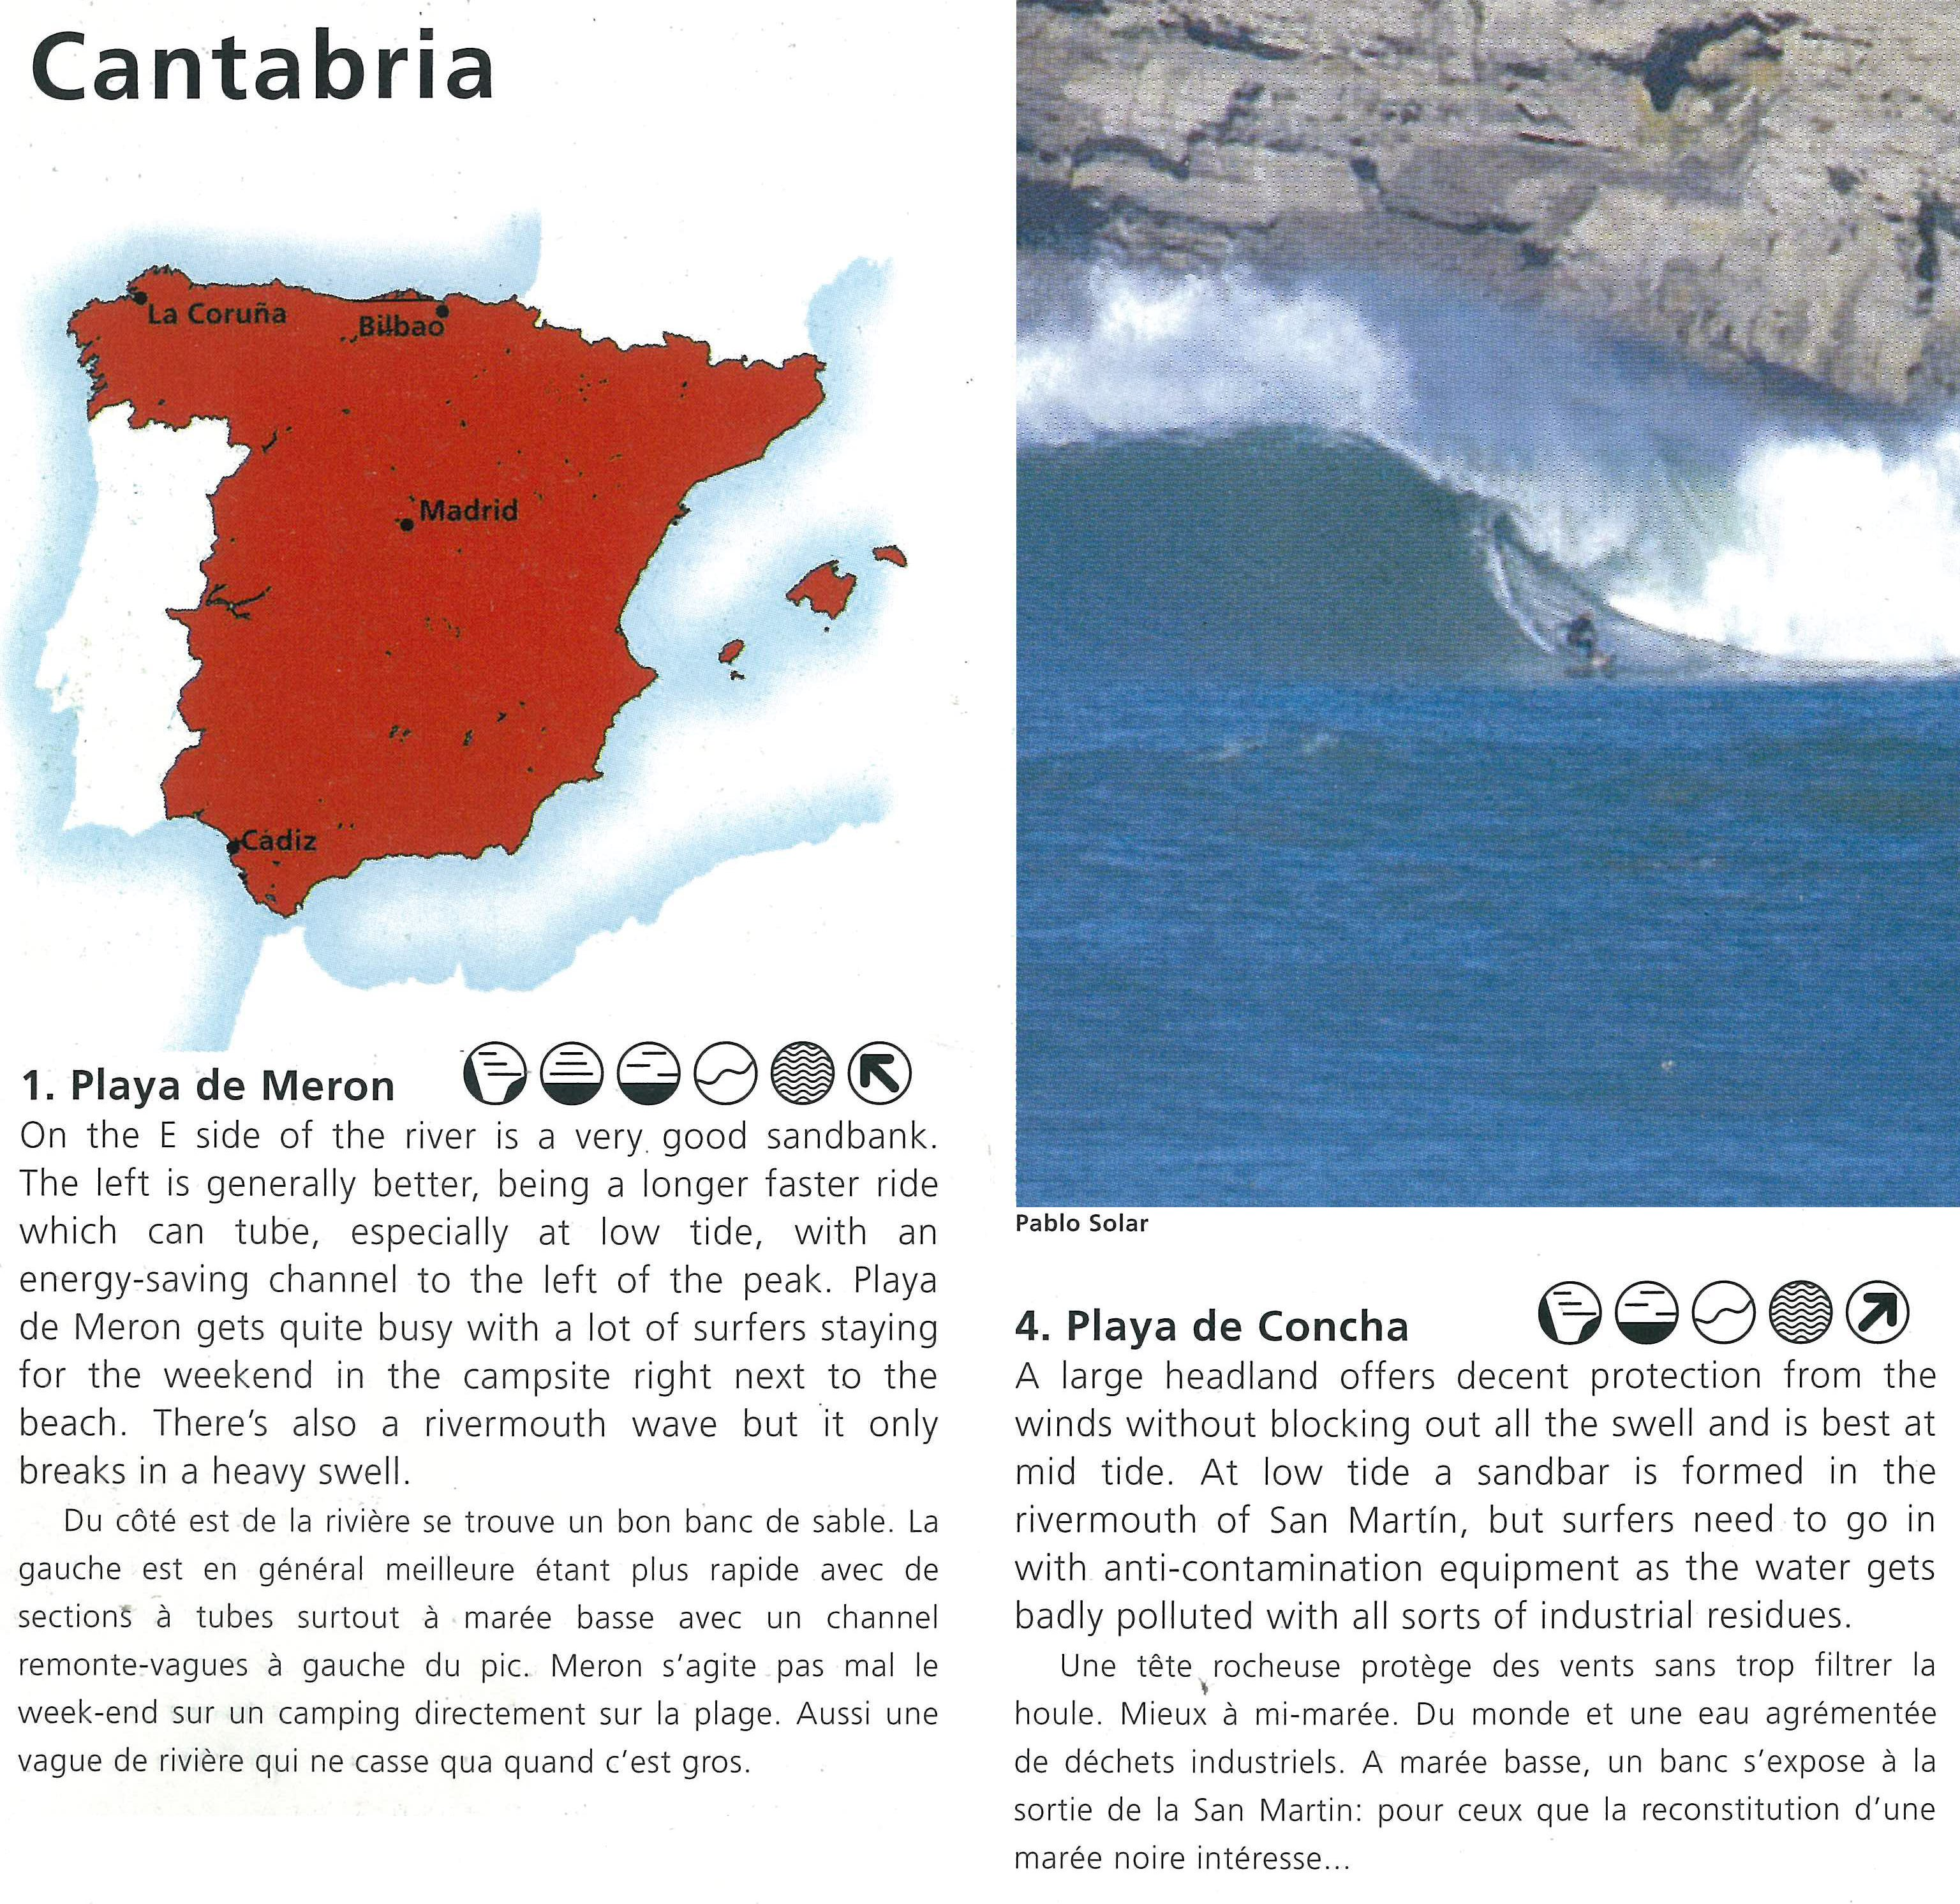
\includegraphics[width=\textwidth]{bilder/spot-descriptions}
  \caption{Spotbeschreibungen der Region Cantabria, Spanien}
  \label{spot-descriptions}
\end{figure}

Ein weiterer Teil eines jeden Kapitels beschäftigt sich mit
Informationen rund um das Reisen. Hier sind sowohl Informationen zur
Einreise in das jeweilige Land, zu den Flughäfen, dem Bus- und Zugnetz
zu finden als auch Telefonnummern von Tourismusbüros, Krankenhäusern
und anderen Einrichtungen. Weiterhin werden Preise für Benzin,
Mietwagen, Unterkunft und Essen angegeben, die zwar nicht immer auf
dem neusten Stand sind, sich aber insbesondere in fremden Ländern als
hilfreich erweisen und als Richtlinie zu verstehen sind. Der Großteil
eines Kapitel im \textit{Stormrider Guide} widmet sich dann den
einzelnen Spots und den dort herrschenden
Surfbedingungen. Beispielsweise wird beschrieben zu welcher Gezeit
bzw. Tide die Wellen an einem Spot am besten brechen, wie stark die
Meeresströmung ist, ob die Brandung an einem Sandstrand oder auf einem
flachen Riff ist oder ob irgendwelche Gefahren zu beachten sind. Jeder
Beschreibung sind zusätzlich Piktogramme zugeordnet, welche die
Surfbedingungen an einem Spot widerspiegeln und einen schnellen
Überblick ermöglichen sollen. In Abbildung \ref{spot-descriptions}
sind z.B. zwei Spotbeschreibungen und die Piktogramme aus der Region
Cantabria in Spanien zu sehen. Um die beschriebenen Spots zu finden,
werden diese in den Reiseführern auf Kartenauschnitten eingezeichnet.

\begin{figure}[h]
  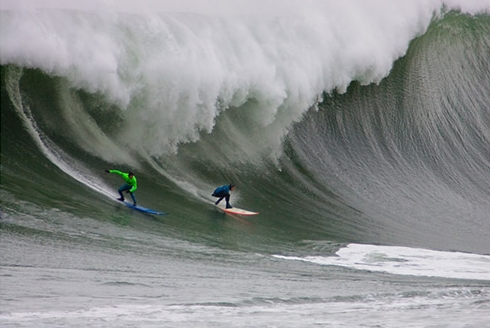
\includegraphics[width=\textwidth]{bilder/mavericks}
  \caption{\textit{''Don't even think about riding big Mavericks''} -
    Kommentar des \textit{World Stormrider Guide} zu
    \textit{Mavericks}, einem bekannten \textit{Big Wave Spot} in
    Nordkalifornien, USA.}
\end{figure}

\section{Swell - Die Entstehung von Wellen}
Die besten Surfspots auf der Welt sind meist in den Ländern zu finden,
in denen regelmäßig \textit{Swell} eintrifft. Mit \textit{Swell} oder
Dünung werden Seewellen bezeichnet, deren Entstehungs\-gebiet weit von
dem Ort entfernt ist, an dem sie später eintreffen und brechen. Swell
wird von den unterschiedlichsten Wetter\-phänomenen erzeugt, zu denen
z.B. Wirbelstürme, Passatwinde, Monsune und Tiefdruckgebiete gehören
\cite[S.15]{storm_europe_1998}. Der in Europa eintreffende Swell
entsteht dabei hauptsächlich durch die Luftzirkulation in
Tiefdruckgebieten über dem Atlantik. Bei ruhigen Wetterverhältnissen
kann man einen größeren Swell sehr gut erkennen, da die eintreffenden
Wellen meist in gleichem Abstand linienförmig angeordnet sind. Diese
linienförmige Anordnung ist z.B. besonders gut in Abbildung
\ref{swell-lines} zu erkennen.

\begin{figure}[h]
 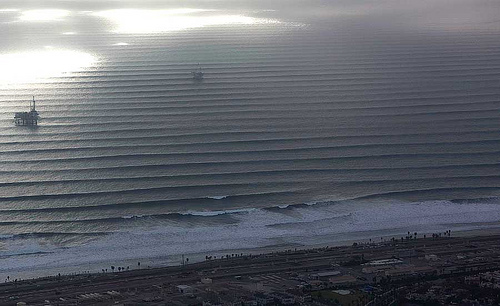
\includegraphics[width=\textwidth]{bilder/swell}
 \caption{Linienförmig eintreffender Swell (Quelle: \textit{Flickr})}
 \label{swell-lines}
\end{figure}

Am Ursprungsort entstehen Wellen dadurch, dass die Wasseroberfläche
durch die über ihr strömenden Winde in Bewegung gesetzt wird. Die
Gipfel und Täler der Wellen werden durch die Zirkulation des Windes
über der Oberfläche immer höher und tiefer, bis sie ein Limit
erreichen und in sich zusammenbrechen. Die Höhe der Wellen ist dabei
von der Stärke, der Dauer und der Strecke, über die der Wind strömt,
abhängig. Die Wellen breiten sich vom Entstehungsort kreisförmig auf
ihre Umgebung im Meer aus. Die Geschwindigkeit der Ausbreitung hängt
dabei von dem Abstand zwischen zwei Wellengipfeln ab, der sogenannten
Wellenlänge. Das Wellenchaos am Entstehungsort mit vielen
unterschiedlichen Wellenlängen beginnt sich mit der Ausbreitung
langsam zu legen. Die schnelleren Wellen, mit weiter auseinander
liegenden Gipfeln, beginnen, die langsameren Wellen zu überholen und
fangen an, sich linienförmig zu ordnen. Die vorderen Wellen werden
dabei zu den kräftiger und linienförmiger angeordneten, die hinteren
Wellen zu den schwächeren und chaotischeren. Je weiter die Strecke,
die ein Swell hinter sich gelegt hat, und je linienförmiger er
geordnet ist, desto größer ist die Geschwindigkeit und die Kraft der
Wellen an dem Ort, an dem sie brechen. Das Eintreffen von Swell ist
eine der Grundvoraussetzungen für gute und surfbare Wellen. Deshalb
gibt es z.B. in Deutschland keine guten Wellen, da der potentiell
eintreffende Swell meist durch England abgeschirmt wird.

\section{Ziel der Diplomarbeit}
Ziel der Diplomarbeit ist die Entwicklung einer \textit{Community
  Plattform} für Surfer, welche den Grundgedanken der
\textit{Stormrider Guides} aufgreift und mit den neuen Möglichkeiten
des Internets und des \textit{Web 2.0} verknüpft. Grundlage der
Plattform sollen Informationen zu den Surfbedingungen an den
verschiedenen Spots sein, die gemeinschaftlich durch die Mitglieder
der Community erstellt und bearbeitet werden können. Diese
Spotbeschreibungen sollen mit aktuellen Wetter- und Wellenvorhersagen
verknüpft und den Nutzern der Plattform zur Verfügung gestellt
werden. Durch die Integration externer Dienste wie \textit{Google
  Maps}, \textit{Flickr} und \textit{YouTube} sollen die bisherigen
Informationen aufgewertet werden. Ziel ist es, eine Plattform zu
entwickeln, auf der für Surfer wichtige Informationen angeboten
werden.

Einige der dabei aufgetretenen Probleme und Lösungen werden in dieser
Arbeit vorgestellt und diskutiert. Im Kapitel \textit{Anforderungen an
  die Web-Applikation} wird auf die Funktionalität der Anwendung und
auf einige der zugrunde liegende Konzepte und Dienste eingegangen. Die
zur Umsetzung verwendeten Technologien und einige nennenswerte
Methoden zur Entwicklung von Web-Applikationen werden anschließend im
Kapitel \textit{Implementierung der Web-Applikation} vorgestellt. Der
Hauptteil beschäftigt sich mit der Integration der Wetter- und
Wellenvorhersagen, die im Kapitel \textit{Aufbau und Analyse der ETL
  Prozesse} näher beschrieben werden. Im Kapitel \textit{Ausblick}
werden schließlich einige Vorschläge gemacht, mit denen die Wetter-
und Wellenvorhersagen verbessert werden könnten, indem die lokalen
Gegebenheiten eines Spots indirekt mit einbezogen werden. Einer dieser
experimentellen Vorschläge bedient sich dabei Verfahren aus dem
Bereich des Data Mining, konnte hier aber wegen fehlenden
Trainingsdaten nicht weiter verfolgt werden.

%%% Local Variables:
%%% mode: latex
%%% TeX-master: "../community-plattform"
%%% End:
